\section{変更のモデル化}

Clojureの焦点はimmutableな値であることを思い出してください。不変のデータでは、"更新 "は、その場のエンティティまたはエンティティを更新するのではなく、エンティティ(またはエンティティのコレクション)の新しいインスタンスを生成します。ほとんどの場合、この方法で十分に目的を果たすことができます。時には、アプリケーションの世界の変化をモデル化し、データの変化を追跡する必要があります。具体的には、変更されたデータのセットへの参照を保持する必要があります。

マルチスレッドのシナリオでは、その場でデータを更新することは、多くの複雑な問題を引き起こします。誰がデータを変更できるのか?他のスレッドにはどのように変更が通知されるのか?複数の更新が同時に発生した場合、どのプロセスが優先されるのか?Clojureは、状態管理ツールによって、これらの質問すべてにエレガントな答えを提供します。これらのツールを効果的に使用するには、まずClojureのアイデンティティと状態へのアプローチを理解する必要があります。

\subsection{スナップショットで見る}

その理解を助けるために、少し時間の話をしましょう。人間の経験は連続的に見えますが、あなたの感覚は情報を個別の量子に分けて収集しています。音、景色、匂いは、それぞれ独立して脳に入り、時間的な瞬間に相関します。その瞬間が連続して再生されることで、連続した知覚が得られると錯覚しているのです。

もし、自分の視覚的な量子を見るなら、次の図に示すエドワード・マイブリッジの「疾走するサリー・ガードナー」のようなスナップショットの連続が見えるだろう。

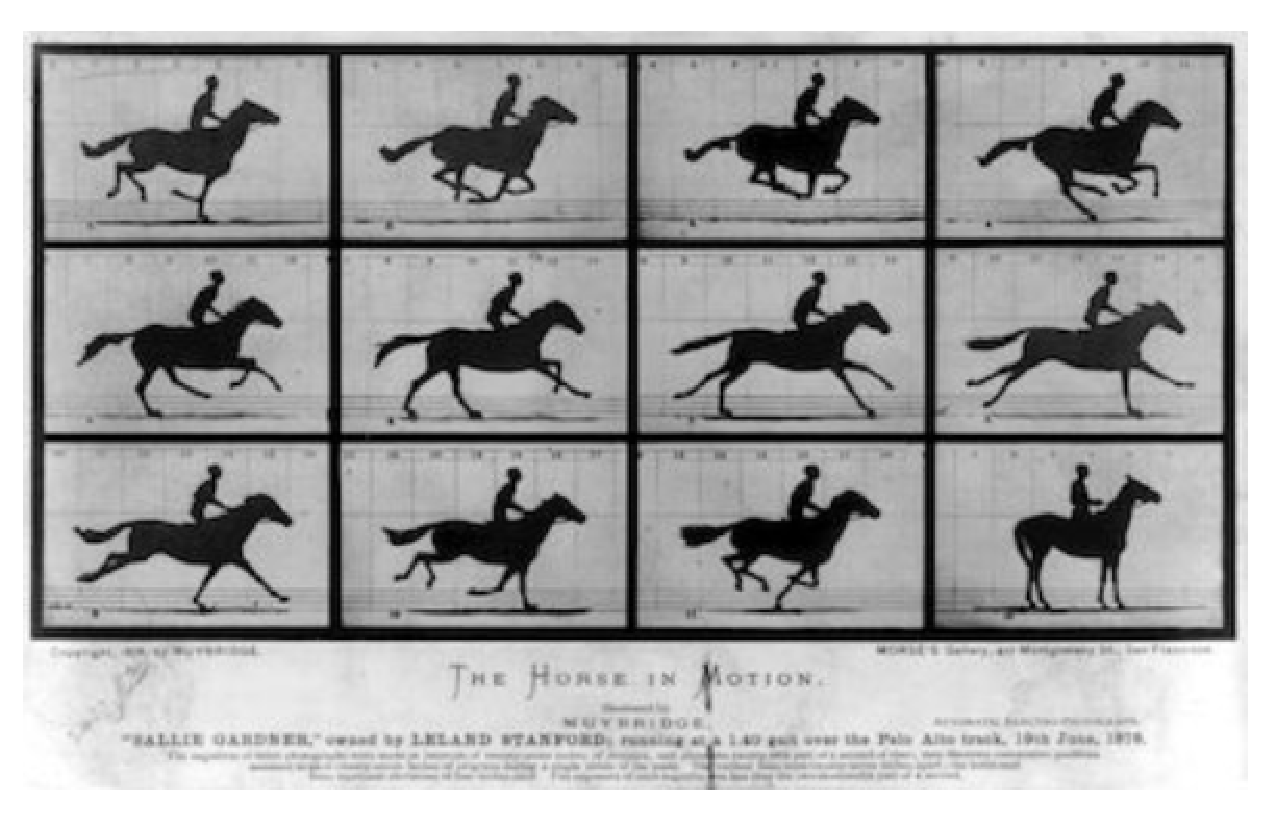
\includegraphics[width=10cm]{fig_04_001.eps}



